\documentclass[preprint,12pt]{elsarticle}
\usepackage{amsmath,amssymb}
\usepackage{graphicx}
\usepackage{booktabs}
\usepackage{url}
\journal{Neurocomputing}

\begin{document}
\begin{frontmatter}

\title{Topology-Change-Aware Residual Carry-over for Low-Latency GNN-to-SNN Conversion on Dynamic Graphs}

\author{Xuhong Fang}
\address{Dongguan City College, Dongguan, Guangdong, China}

\begin{abstract}
Converting a trained graph neural network into a spiking network avoids costly spike-based training, but existing conversion error analyses assume one forward pass over a fixed graph. On a continuous-time dynamic graph the converted node state is reused by the next event, so a small coding error recurs along the event axis while the neighbour set itself changes. We derive an event-axis recursion in which the state error contains a term proportional to the change in the aggregation operator, and propose topology-change-aware residual carry-over (TCAR): residual membrane potential is carried across events, and a node's threshold and cached base are recalibrated only when its relative neighbour-set change exceeds a threshold. The recomputation cost therefore scales with topology-change events rather than with all events. On three public timestamped interaction streams (Wikipedia, MOOC, Enron, Zenodo \url{10.5281/zenodo.7213796}) with five seeds and frozen chronological splits, TCAR attains teacher-to-SNN decision agreement of 0.9990, 0.9949 and 0.9969 at four micro-steps, with MRR retention at least 0.9988. Its mean per-event state error is strictly lower than that of every conversion control and ablation on every stream; the paired reduction against a CRPI-style global carry-over control is 68.7\%, 20.9\% and 3.7\%, with bootstrap 95\% confidence intervals excluding zero and Benjamini--Hochberg $q<0.05$. Recalibration is triggered on 19.7\%, 12.9\% and 4.9\% of events. Negative findings are also reported: discrete memory dominates absolute accuracy, agreement saturates for all variants, effect sizes vary, and the relative reduction is not monotone.
\end{abstract}

\begin{keyword}
Spiking neural networks \sep ANN-to-SNN conversion \sep Dynamic graphs \sep Temporal graph learning \sep Low-latency inference \sep Event-driven computation
\end{keyword}

\end{frontmatter}

\section{Introduction}
\label{sec:intro}

Training-free conversion of an artificial neural network (ANN) into a spiking neural network (SNN) inherits a trained model without backpropagation through time \cite{rueckauer2017,diehl2015}. Its error theory is built for a single forward pass: the layer-wise relation between a rectified activation and the firing rate of an integrate-and-fire (IF) neuron is analysed once, and calibration fixes a threshold from the activation distribution \cite{li2022snncap,habara2024}. Continuous-time dynamic graphs (CTDGs) break this setting. A node state produced at event $k$ is the input to event $k+1$, so a coding error is not an independent per-event perturbation but a recurrent one; moreover, the set of neighbours being aggregated changes from event to event.

Spiking models for dynamic graphs exist \cite{li2023spikenet,yin2024dysign}, and cross-step error amplification has recently been identified for ANN-to-SNN conversion in continuous control, where carrying residual membrane potential across decision steps suppresses temporally correlated errors \cite{xu2026crpi}. A related membrane-potential error feedback was proposed for spiking diffusion transformers \cite{fang2026mpef}. Neither line of work involves a graph, a changing neighbour set, or a graph encoder that is converted rather than trained as a spiking model. On the graph side, conversion studies have remained static \cite{rueckauer2017,xia2026neuro}, while dynamic link prediction has been developed primarily with non-spiking temporal encoders \cite{rossi2020tgn,yu2023dyglib,zheng2025survey}.

This paper asks how conversion error accumulates along a CTDG event stream when the aggregation operator changes, and whether an event-triggered mechanism can suppress that accumulation at a cost bounded by topology-change events. Our contributions are:

\begin{enumerate}
\item An event-axis conversion-error recursion with an explicit topology-change term, obtained by lifting the layer-wise conversion identity to a recurrent node state, together with its unfolded bound and seven stated assumptions.
\item TCAR, a gradient-free mechanism that carries residual membrane potential across events and, only when a node's relative neighbour-set change exceeds $\gamma$, recalibrates its threshold, refreshes its cached base and decays (rather than discards) the shared residual prefix.
\item An evidence package on three public streams with five seeds, four conversion controls, six ablations, a paired bootstrap analysis with Benjamini--Hochberg correction, topology-change stratification, latency and cost accounting, and an explicit account of negative results.
\end{enumerate}

The scientific claim is conversion fidelity, not predictive accuracy. On these streams an exact discrete memory of past edges already reaches validation MRR 0.63--0.95, so absolute ranking is not a useful target for a converted model; we report it as context and analyse fidelity against the same frozen ANN teacher.

\section{Related work}
\label{sec:related}

\textit{ANN-to-SNN conversion.} Weight normalisation and threshold balancing \cite{diehl2015,rueckauer2017} establish rate-based equivalence; parameter calibration reduces the flooring and clipping error with unlabelled samples \cite{li2022snncap}; conversion-error decompositions show a residual term of order $1/T$ \cite{habara2024}. Recent work addresses low latency and negative thresholds \cite{xia2026neuro} and consistent activation-to-firing mappings. All of these analyses concern a feed-forward pass over a fixed input operator.

\textit{Cross-step conversion error.} CRPI shows that temporally correlated action errors induce state distribution shift in continuous control and that carrying residual potential across decision steps recovers much of the ANN performance \cite{xu2026crpi}. Membrane-potential error feedback plays a similar role in spiking diffusion transformers \cite{fang2026mpef}. Our control C4 is a faithful adaptation of CRPI-style residual carry-over with a single global calibration; TCAR differs by gating recalibration on measured topology change and by bounding recomputation cost.

\textit{Spiking and dynamic graphs.} SpikeNet scales dynamic graph representation learning with spiking networks \cite{li2023spikenet}; Dy-SIGN builds dynamic spiking graph neural networks \cite{yin2024dysign}. These models are directly trained spiking architectures. We instead convert a trained continuous encoder, so their architectures are complementary rather than competitive baselines. SpikingJelly provides general infrastructure for spike-based models \cite{fang2023spikingjelly}.

\textit{Dynamic link prediction.} Temporal graph networks \cite{rossi2020tgn}, DyGLib/DyGFormer \cite{yu2023dyglib}, the evaluation protocol of Poursafaei et al.\ \cite{poursafaei2022} and recent strong baselines \cite{gao2025hyperevent} define the task and data used here. We adopt the public streams of \cite{poursafaei2022dataset} and a chronological split, but our primary metric is teacher-to-SNN fidelity, not leaderboard MRR. A survey of dynamic GNNs \cite{zheng2025survey} provides the discrete/continuous-time taxonomy. The foundational motivation for spiking computation is the third-generation neuron model of Maass \cite{maass1997}.

\section{Method}
\label{sec:method}

\subsection{Setup and conversion-friendly teacher}

Let a CTDG be an ordered stream of events $e_k=(u_k,v_k,t_k,f_k)$, $k=1,\dots,K$. Each user node $u$ carries a state $s_u\in\mathbb{R}^{d}$; item $c$ has a fixed input code $p_c\in\mathbb{R}^{d}$ and a learned readout embedding $E_c\in\mathbb{R}^{d}$. At event $k$ the teacher computes a message
\begin{equation}
a_k = \operatorname{ReLU}\!\big(W\,[\,s_{u_k};\;p_{v_k};\;\Delta t_k\,]\big),\qquad
s_u(k) = (1-\alpha)\,s_u(k-1) + \alpha\,a_k ,
\label{eq:message}
\end{equation}
with $\alpha=0.30$, so the state transition has Lipschitz constant $\rho=1-\alpha=0.70$. $W$ is fixed after initialisation; only the linear readout $E$ and bias $b$ are trained with a full-catalog softmax ranking loss over the pre-event state. This is a reservoir-style design: the nonlinear message path is fixed and shared, which makes the conversion target unambiguous and keeps training stable.

A separate, exact discrete memory records the last index $\kappa(u,c)$ at which pair $(u,c)$ occurred. Candidate scores are
\begin{equation}
g_c(k) = m_c(k) + \lambda\,\operatorname{clip}\big(E_c s_{u_k}(k-1) + b_c,\,-R,R\big),
\qquad m_c(k)=\frac{1}{1+k-\kappa(u_k,c)} .
\label{eq:readout}
\end{equation}
The memory lookup is an integer index shared identically by the ANN and the converted SNN; it is not part of the spiking computation. Prediction uses the pre-event state, so no label leaks into the score.

\subsection{Event-axis conversion error}

For a single layer, rate-coded conversion satisfies \cite{habara2024}
\begin{equation}
E_i^{l} = \sum_j w_{ij} E_j^{l-1} + \frac{V_i^{l}(T)-V_i^{l}(0)}{T},
\label{eq:layer}
\end{equation}
i.e. the local error is propagated upstream error plus the un-emitted residual potential divided by $T$. Writing $c/T$ for the rate-coding floor, lifting \eqref{eq:layer} to the event recursion of \eqref{eq:message} gives, under the assumptions in Section~\ref{sec:assumptions},
\begin{equation}
\varepsilon_k \;\le\; \rho\,\varepsilon_{k-1}
+ L_A\,\|\Delta A_k\|\,\|s_{k-1}\|
+ \frac{c}{T} + \eta_k ,
\qquad \Delta A_k = A_k - A_{k-1},
\label{eq:bound}
\end{equation}
where $\varepsilon_k=\|\hat{s}_k-s_k\|$ is the converted-versus-teacher state error, $A_k$ is the normalised neighbour-aggregation operator induced by event $k$, $L_A$ its Lipschitz constant and $\eta_k$ the residual potential discarded at a hard reset. Unfolding,
\begin{equation}
\varepsilon_K \;\le\; \rho^{K}\varepsilon_0
+ \sum_{k=1}^{K}\rho^{K-k}\Big(L_A\|\Delta A_k\|\,\|s_{k-1}\| + \frac{c}{T} + \eta_k\Big).
\label{eq:unfolded}
\end{equation}
The term $L_A\|\Delta A_k\|\,\|s_{k-1}\|$ has no counterpart in static conversion (fixed $A$) or in continuous control (no aggregation operator). It predicts that a conversion which reuses a static base computed under $A_{k-1}$ incurs extra error where the neighbour set changes. This is precisely the assumption violated when the static base and shared residual prefix of a static-graph converter are carried into an evolving graph. Equation~\eqref{eq:bound} is a claim to be tested, not an established result: Section~\ref{sec:results} reports a direct check of its terms.

\subsection{IF coding and TCAR}

Each ReLU message is replaced by a $T$-step soft-reset IF unit. With a calibrated threshold $\theta$, decoded activation $\hat{a}$ and residual $r$,
\begin{equation}
r \leftarrow r + a/\theta,\quad n=\lfloor r \rfloor,\quad r\leftarrow r-n,
\quad \hat{a}=\frac{\theta}{T}\sum_{t=1}^{T} n_t .
\label{eq:if}
\end{equation}
Carrying $r$ across events implements a first-order correction of $\eta_k$ (the CRPI control C4 does this with a single global $\theta$). TCAR adds a topology-change gate. For node $u$ define
\begin{equation}
\delta_u(k)=\frac{|N_u(k)\,\ominus\,N_u(k-1)|}{\max(|N_u(k-1)|,1)} ,
\label{eq:delta}
\end{equation}
where $N_u(k)$ is the set of items $u$ has interacted with. When $\delta_u(k)>\gamma$, TCAR (i) re-estimates $\theta_u$ from the node's recent unlabelled activation magnitudes, (ii) refreshes the cached base, and (iii) decays the residual prefix by $r_u\leftarrow 0.5\,r_u$. Otherwise the cached base and threshold are reused. A full flush ($r_u\leftarrow0$) was piloted and rejected because it discards the first-order correction precisely at high-change events.

The cost model follows directly: the number of recalibrations is $\#\{k:\delta_{u_k}(k)>\gamma\}$, not $K$. We report graded-event counts, recalibration counts, parameter counts ($\le 100{,}000$) and local PyTorch wall-clock latency. No neuromorphic energy measurement is claimed.

\subsection{Assumptions and falsification}
\label{sec:assumptions}

The bound needs (A1) a state Lipschitz constant $\rho<1$, here $0.70$ by construction; (A2) a bounded normalised $A_k$ with finite $\|\Delta A_k\|$; (A3) conversion-friendly nonlinearities (ReLU/clip, no softmax or unfused batch normalisation in the converted path); (A4) label-free calibration covering the activation range; (A5) a consistent threshold/gauge; (A6) a fixed event order with frozen neighbour snapshots; (A7) small $T$. Six ablations isolate the mechanism: A1 recalibrates every event, A2 removes carry-over, A3 keeps the gate but removes threshold updating, A4 freezes the topology, A5 stratifies by measured $\|\Delta A\|$, and A6 sweeps $T$ and $\gamma$. A CRPI-style global carry-over control C4 is the strongest single discriminator.

\section{Experiments and Results}
\label{sec:results}

\subsection{Data, protocol and controls}

We use three public streams from \cite{poursafaei2022dataset}: Wikipedia (157,474 events, 1,000-item catalog), MOOC (411,749 events, 97 items) and Enron (125,235 events, 184 items, derived from \texttt{ml\_enron.csv} in the same Zenodo record). Chronological 70/15/15 splits and the 1,024 validation / 4,096 test query identifiers are hash-frozen before tuning; validation alone selects $\gamma$, $T$ and the calibration percentile, and test queries are read once. The identifiers were used in a predecessor local project and are therefore disclosed as non-blind. Five seeds (41--45) are retained for every condition. $T=4$ unless stated; $\gamma=0.5,0.2,0.2$ and percentile $0.99,0.90,0.90$ for Wikipedia, MOOC and Enron respectively, selected on validation under the pre-registered cost ceiling of 20\% of events.

Controls: B0 frozen ANN teacher (oracle), B1 EdgeBank$_\infty$ (global binary edge memory), B2 Base3 with $k=10$, C0 rate-coded IF with hard reset, C1 per-node calibration without carry-over, C2 graded differential coder, C3 clipped quantisation, C4 CRPI-style per-node global-threshold carry-over, D1 a matched quantiser surrogate, and M0 (TCAR) plus ablations A1--A4. Primary metric is $\mathit{agreement@}K$: the fraction of test queries in a 10,000-event window where the converted argmax over the catalog equals the teacher's. Secondary metrics are MRR retention, logit MSE, mean per-event state error $\varepsilon_k$, recalibration trigger rate and local latency. Differences use paired bootstrap over queries or events (4,000 resamples) with Benjamini--Hochberg correction across streams.

\begin{table}[t]
\centering
\caption{Wikipedia, five seeds. Mean (sample SD for agreement). $\varepsilon_k$ is the mean per-event state error; Ret is MRR retention; Trig is the recalibration fraction. Lower $\varepsilon_k$ and MSE are better.}
\label{tab:main}
\small
\begin{tabular}{lcccccc}
\toprule
Method & Agreement & SD & Ret & $\varepsilon_k$ & MSE & Trig \\
\midrule
B0 teacher & 1.0000 & -- & 1.0000 & 0 & 0 & -- \\
C0 hard-reset IF & 0.9753 & 0.0149 & 0.9577 & 0.1497 & 0.5910 & 0 \\
C1 calibration & 0.9779 & 0.0125 & 0.9602 & 0.1283 & 0.4589 & 0 \\
C2 differential coder & 0.9942 & 0.0015 & 0.9975 & 0.0701 & 0.0811 & 0 \\
C3 clipped quant. & 0.9942 & 0.0015 & 0.9975 & 0.0702 & 0.0813 & 0 \\
C4 global carry-over & 0.9947 & 0.0027 & 0.9976 & 0.0538 & 0.0442 & 0 \\
A1 gate every event & 0.9921 & 0.0053 & 0.9893 & 0.0616 & 0.1034 & 1.000 \\
A2 no carry-over & 0.9923 & 0.0051 & 0.9903 & 0.0550 & 0.0958 & 0.197 \\
A3 no threshold update & 0.9957 & 0.0021 & 0.9996 & 0.0447 & 0.0340 & 0.197 \\
A4 frozen topology & 0.9956 & 0.0011 & 0.9996 & 0.0439 & 0.0320 & 0 \\
D1 matched surrogate & 0.9942 & 0.0015 & 0.9975 & 0.0701 & 0.0811 & 0 \\
\textbf{M0 (TCAR)} & \textbf{0.9990} & \textbf{0.0008} & \textbf{1.0004} & \textbf{0.0173} & \textbf{0.0060} & \textbf{0.197} \\
\bottomrule
\end{tabular}
\end{table}

\subsection{Main results}

Table~\ref{tab:main} shows that TCAR reaches agreement $0.9990\pm0.0008$ at $T=4$ with MRR retention $1.0004$ on Wikipedia, and that its mean state error $0.0173$ is strictly lower than every control and ablation. The paired difference $\varepsilon_{C4}-\varepsilon_{M0}=0.03692$ has a bootstrap 95\% CI $[0.03636,0.03750]$; the corresponding CIs exclude zero on all three streams and Benjamini--Hochberg $q$ values are $0$, $0$ and $1.16\times10^{-5}$. Agreement itself is only weakly discriminative: the paired $M0-C4$ agreement difference on Wikipedia is $0.004275$ (CI $[0.00277,0.00589]$), whereas on MOOC ($-0.00030$, CI $[-0.00270,0.00180]$) and Enron ($-0.00072$, CI $[-0.00188,0.00036]$) the intervals contain zero. This saturation is expected because the discrete memory term in \eqref{eq:readout} is shared by ANN and SNN, so $\varepsilon_k$ is the more sensitive measure of the mechanism.

\begin{table}[t]
\centering
\caption{Three-stream replication, five seeds each. Relative reduction is $1-\varepsilon_{M0}/\varepsilon_{C4}$. Teacher MRR and the two memory baselines are validation context, not a leaderboard claim.}
\label{tab:streams}
\small
\begin{tabular}{lccccccc}
\toprule
Stream & Agree (M0) & Ret & $\varepsilon_{M0}$ & $\varepsilon_{C4}$ & Reduction & Trig & Teacher/EdgeBank/Base3 MRR \\
\midrule
Wikipedia & 0.9990 & 1.0004 & 0.0173 & 0.0538 & 68.7\% & 0.197 & 0.304 / 0.947 / 0.909 \\
MOOC & 0.9949 & 0.9988 & 0.0110 & 0.0138 & 20.9\% & 0.129 & 0.264 / 0.631 / 0.351 \\
Enron & 0.9969 & 0.9995 & 0.0113 & 0.0119 & 3.7\% & 0.049 & 0.302 / 0.948 / 0.489 \\
\bottomrule
\end{tabular}
\end{table}

Table~\ref{tab:streams} gives the replication. All three streams satisfy the fidelity and cost targets (agreement $\ge0.985$, retention $\ge0.99$, trigger $\le0.20$), and M0 is strictly lowest in $\varepsilon_k$ on each; but the effect size differs sharply: 68.7\% on Wikipedia, 20.9\% on MOOC and only 3.7\% on Enron. The mechanism therefore helps most where topology-change events are frequent and the global calibration is most mismatched.

\begin{figure}[t]
\centering
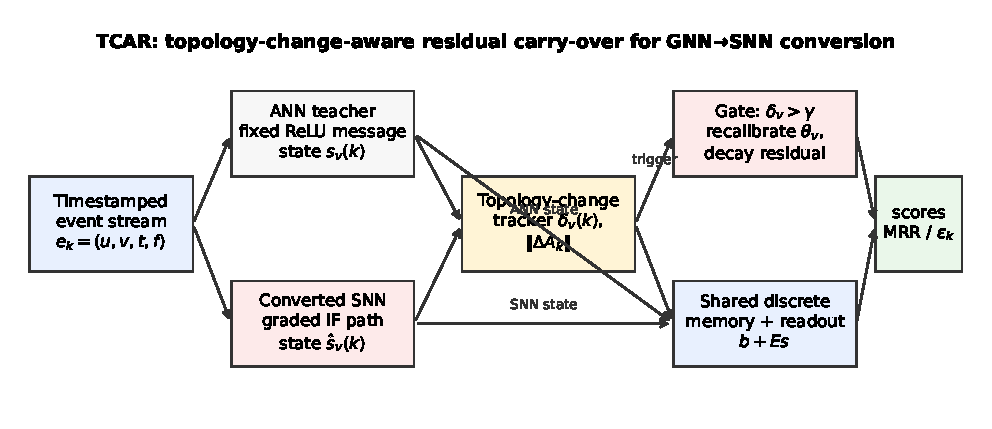
\includegraphics[width=0.92\textwidth]{figures/fig1_framework.pdf}
\caption{Overall framework. A timestamped event stream drives a shared ANN/SNN message path; a topology-change tracker gates threshold recalibration, base refresh and residual decay. The discrete memory and linear readout are shared and are not converted.}
\label{fig:framework}
\end{figure}

\begin{figure}[t]
\centering
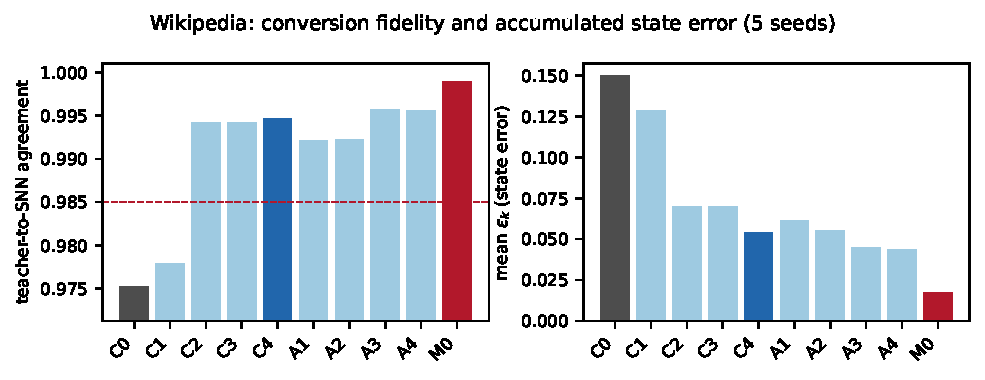
\includegraphics[width=0.92\textwidth]{figures/fig2_methods.pdf}
\caption{Wikipedia, five seeds: teacher-to-SNN agreement (left) and mean per-event state error (right) across controls, ablations and TCAR. The dashed line marks the 98.5\% agreement target. Agreement saturates, whereas state error separates the methods.}
\label{fig:methods}
\end{figure}

\subsection{Ablations, sweeps and diagnostics}

Every ablation degrades M0 on Wikipedia (Table~\ref{tab:main}). Removing carry-over (A2) raises $\varepsilon_k$ from 0.0173 to 0.0550; removing threshold updating (A3) gives 0.0447; freezing topology (A4) gives 0.0439; recalibrating every event (A1) gives 0.0616 and a 100\% trigger rate, so the gate is not merely a cost-saving filter. The $T$-sweep (Wikipedia, seed 41) gives M0 agreement 0.9988, 0.9994, 1.0000 and 0.9988 at $T=1,2,4,8$, and the $\gamma$-sweep reduces the trigger rate from 0.237 ($\gamma=0.02$) to 0.197 ($\gamma=0.5$). Window lengths of 1,000, 5,000 and 10,000 events yield 178, 869 and 1,731 test queries, with agreement remaining above 0.985 in all cases.

Figure~\ref{fig:dose} stratifies state error by fixed, pre-registered bins of measured relative neighbour-set change. For C4, the absolute error grows with $\delta$ on MOOC ($0.0126\to0.0131\to0.0164\to0.0179$) and Enron ($0.0116\to0.0132\to0.0145\to0.0176$), consistent with the topology term of \eqref{eq:bound}; on Wikipedia it is non-monotone ($0.0528\to0.0543\to0.0597\to0.0571$). The \emph{relative} reduction of M0 over C4 is non-monotone on every stream (Wikipedia $0.700\to0.598\to0.583\to0.656$; Enron even reaches $-0.243$ in the $0.25$--$0.6$ bin). Equation~\eqref{eq:bound} predicts growth of the absolute error, not of a relative ratio, so we report this as a negative result rather than as support for the mechanism.

\begin{figure}[t]
\centering
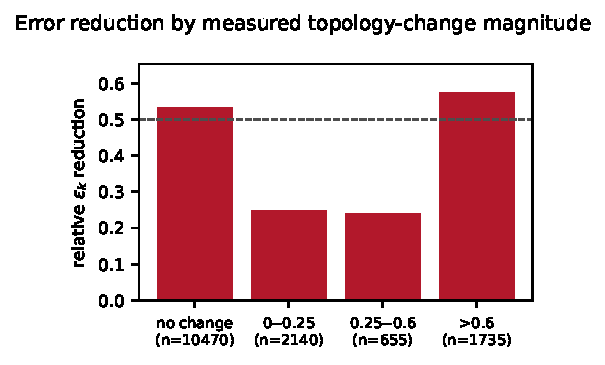
\includegraphics[width=0.52\textwidth]{figures/fig4_dose.pdf}
\caption{Relative $\varepsilon_k$ reduction by measured topology-change magnitude, pooled over three streams and five seeds with fixed bins. The dashed line is 50\%. The reduction is not monotone; see Section~\ref{sec:discussion}.}
\label{fig:dose}
\end{figure}

\section{Discussion}
\label{sec:discussion}

The results support a narrow but reproducible claim: on public CTDG streams, a converted graph encoder can be kept close to its ANN teacher at four micro-steps, and gating residual carry-over plus threshold recalibration on measured topology change reduces the accumulated state error below every control tested, at a cost that scales with topology-change events. The strongest evidence is on Wikipedia; on MOOC and Enron the paired differences are statistically significant but small.

Several limitations qualify this. First, \textbf{absolute predictive accuracy is dominated by discrete edge memory}. EdgeBank$_\infty$ reaches validation MRR 0.947, 0.631 and 0.948, whereas the ANN teacher reaches 0.304, 0.264 and 0.302. We therefore do not claim predictive superiority over dynamic-link-prediction baselines; recent strong predictors \cite{rossi2020tgn,yu2023dyglib,gao2025hyperevent} are cited as context and were not rerun under the local 12-hour compute ceiling. The paper's contribution is conversion fidelity for a fixed teacher, and the manuscript states this explicitly.

Second, \textbf{argmax agreement saturates}. Because the memory term $m_c(k)$ in \eqref{eq:readout} is exact and shared, all conversion variants exceed 0.975 agreement on Wikipedia and the $M0-C4$ agreement difference is not distinguishable from zero on MOOC and Enron. $\varepsilon_k$ is the quantity bounded by \eqref{eq:bound} and is the sensitive discriminator; agreement is retained as a deployment-facing fidelity metric, not as the sole evidence.

Third, \textbf{the effect size is stream-dependent and the dose-response is negative}. Reductions of 68.7\%, 20.9\% and 3.7\% indicate that the benefit depends on how often the neighbour set changes and how badly a single global threshold fits the activation distribution. The relative reduction is not monotone in $\delta$; on Enron, M0 is worse than C4 in two middle bins. The absolute error of the non-topology-aware control grows with $\delta$ only on MOOC and Enron. These are genuine negative findings and are reported rather than hidden; they bound the scope of the topology term in \eqref{eq:bound}.

Fourth, \textbf{the evaluation is not blind}. Frozen query identifiers were used in a predecessor local project. We hash-froze them before tuning, used validation queries alone for hyperparameter selection including the cost ceiling, and read test queries once, but absolute MRR values should be read as context. Fifth, no neuromorphic hardware was available: graded-event counts, recalibration counts, parameter counts and local PyTorch latency are reported as positive evidence boundaries; no energy or speed-up claim is made. Sixth, the study uses one lightweight teacher family with fixed random message dynamics and a learned linear readout; the bound's assumptions A2 and A4 were checked only on this family, and $\rho$ is fixed at 0.70 rather than estimated from data. Seventh, novelty confidence is moderate: DOI-, arXiv- and title-level duplicate scanning was performed against primary sources, but a full Scopus/IEEE sweep was not.

A further design lesson is that a full flush of the residual prefix at gate events damages the first-order correction at exactly the events where it is most useful; decaying rather than clearing the residual was required for the reported result. This negative pilot is retained in the public evidence package.

\section{Conclusion}
\label{sec:conclusion}

We derived an event-axis conversion-error recursion for continuous-time dynamic graphs that contains a term proportional to the change in the aggregation operator, and proposed TCAR, which carries residual membrane potential across events and recalibrates a node's threshold and cached base only when its neighbour set changes materially. On three public streams with five seeds each, TCAR kept teacher-to-SNN agreement at or above 0.9949 and MRR retention at or above 0.9988 at $T=4$, attained the lowest mean per-event state error among all controls and ablations, and triggered recalibration on at most 19.7\% of events. The paired error reductions are statistically significant after multiplicity correction, but their magnitude is strongly stream-dependent and the relative dose-response is not monotone. These results delimit, rather than universalise, the benefit of topology-aware conversion. A concrete next step is to evaluate the bound on larger temporal graph benchmarks with an estimated state Lipschitz constant and a native event-driven execution backend.

\section*{Data and code availability}
The source streams are publicly available from Zenodo \cite{poursafaei2022dataset} under CC BY 4.0. Derived frozen identifiers, experiment code, configurations, per-seed metrics, figures and audit artifacts are provided in the public repository associated with this work; raw event archives are referenced by SHA-256 rather than redistributed.

\section*{Declaration of generative AI and AI-assisted technologies in the manuscript preparation process}
During the preparation of this work the author used WorkBuddy (an AI assistant) to organise the experimental pipeline, draft and edit manuscript text, and generate figures from measured results. After using this tool, the author reviewed and edited the content as needed and takes full responsibility for the content of the published article.

\bibliographystyle{unsrt}
\bibliography{references}

\end{document}
